\chapter{Validation}
\label{chap:validation}

\section{Introduction}

This chapter unfolds as a meticulous exploration into the performance and reliability of the Fair-by-Design workflow. To conduct a thorough assessment, the well known dataset Adult has been strategically chosen as the testing ground. The dataset, rich in socioeconomic and demographic attributes, provides a robust platform for evaluating the workflow's effectiveness across various machine learning algorithms.

The central emphasis of this validation endeavor is to ascertain not only the accuracy and predictive capabilities of the implemented models but also the extent to which the Fair-by-Design workflow succeeds in fostering fairness. The Adult dataset allows for a nuanced examination of how different algorithms respond to the intricacies of real-world data, shedding light on the interplay between accuracy and fairness.

Throughout this chapter, the validation process unfolds systematically, encompassing diverse algorithms applied to the dataset. The goal is to detect both the strengths and potential limitations of the Fair-by-Design approach, providing valuable insights for its application in scenarios where the equitable treatment of individuals and the accuracy of predictions are of paramount importance. The subsequent sections detail the experimental setup, algorithmic choices, and the rigorous evaluation metrics employed to ensure a comprehensive understanding of the Fair-by-Design workflow's performance on the chosen dataset.

\section{Objective definition}
\label{section:val_obj}

In this section, are precicely outlined the objectives guiding the Fair-by-Design workflow, focusing on effective income prediction while addressing fairness and mitigating biases. The key components include the identification of protected attributes, selection of fairness notions, and corresponding fairness metrics.

\subsection{Prediction Objective}

\begin{itemize}
    \item Goal: Classify in a fairness way if an individual earns more or less than 50,000\$ / year.
\end{itemize}

\subsection{Protected Attributes}

\begin{itemize}
    \item Attributes: "Ethnicity" and "Sex"
\end{itemize}

\subsection{Fairness Notions}

\begin{itemize}
    \item Demographic Parity:
    \begin{itemize}
        \item Objective: Ensure consistent distribution of predicted outcomes across different subgroups based on protected attributes.
    \end{itemize}
    
    \item Group Fairness:
    \begin{itemize}
        \item Objective: Guarantee equitable predictions within specific subgroups defined by protected attributes.
    \end{itemize}
\end{itemize}

\subsection{Fairness Metrics}

\begin{itemize}
    \item For Demographic Parity:
    \begin{itemize}
        \item Metric: Disparate Impact
    \end{itemize}
    
    \item For Group Fairness:
    \begin{itemize}
        \item Metric: Demographic Parity Difference
    \end{itemize}
\end{itemize}

These succinctly defined objectives, paired with chosen fairness notions and metrics, lay the groundwork for the  workflow, ensuring a focused approach toward accurate predictions while fostering fairness across diverse subgroups.

\section{Data collection}
\label{section:val_dc}

The dataset is already divided into two sets:
\begin{itemize}
    \item \emph{Training set}: 32,561 items
    \item \emph{Test set}: 16,281 items
\end{itemize}

There are 14 independent features of different types and one dependent variable. Each record represents one individual and the output represents if the individual earns more or less than 50,000\$ on year basis.

The two protected attributes detected in \cref{section:val_obj} are both discrete ones, while a consideration useful for the next steps is related to the output variable. This attribute is a binary one, but it is represented as a string. So it's important to ensure that the encoding in both training and test set are the same.

\section{Data pre-processing}

Starting from the information provided by \cref{section:val_dc} in this section all the variables represend as string as been labeled the same manner. This led to a consistent dataset to be used in the models training.

\section{Algorithm design}
\label{section:val_alg}

In the context of the Fair-by-Design workflow, six key fairness algorithms have been strategically chosen to comprehensively test the workflow's effectiveness. Each algorithm serves a specific purpose within the workflow, contributing to the overarching goal of achieving fairness in predictions.

\subsection{Pre-processing Algorithms}

\subsubsection{Data Augmentation Algorithm}

\begin{itemize}

    \item \emph{Algorithm Description:} The proposed data augmentation algorithm introduces synthetic samples to the training dataset. By augmenting the data, especially focusing on underrepresented groups, the algorithm aims to enhance the model's exposure to diverse scenarios, promoting a more robust understanding of the underlying patterns.

    \item \emph{Reasoning:} Data augmentation is crucial for addressing imbalances in the training data, allowing the model to generalize better across different groups and mitigating biases stemming from insufficient representation.

\end{itemize}

\subsubsection{Fairness Through Unawareness}

\begin{itemize}

    \item \emph{Algorithm Description:} Fairness through unawareness involves deliberately avoiding the use of sensitive attributes in the modeling process. This pre-processing approach aims to promote fairness by excluding potentially biased features, thus reducing the risk of discrimination based on sensitive attributes.

    \item \emph{Reasoning:} Fairness through unawareness is considered to mitigate biases by preventing the model from directly using sensitive attributes, thereby minimizing the potential for biased predictions associated with these attributes.

\end{itemize}

\subsection{In-processing Algorithms}

\subsubsection{ExponentiatedGradient}

\begin{itemize}

    \item \emph{Algorithm Description}: The ExponentiatedGradient algorithm applies iterative re-weighting to the training data, seeking to find a fair classifier by minimizing the disparity in predictions across sensitive groups.

    \item \emph{Reasoning:} ExponentiatedGradient is chosen for its versatility and effectiveness in in-processing fairness. It provides a fine-tuning mechanism during training to achieve parity in predicted outcomes.

\end{itemize}

\subsubsection{GridSearch}

\begin{itemize}

    \item \emph{Algorithm Description:} GridSearch is a generic algorithm that explores a range of hyperparameter values to find the optimal configuration for a fair classifier.

    \item \emph{Reasoning:} GridSearch is included to assess the impact of hyperparameter tuning on fairness outcomes, offering insights into the versatility of the approach.

\end{itemize}

\subsection{Post-processing Algorithms}

\subsubsection{ThresholdOptimizer}

\begin{itemize}

    \item \emph{Algorithm Description:} ThresholdOptimizer focuses on adjusting decision thresholds post-modeling to achieve fairness goals. It provides flexibility in fine-tuning predictions without retraining the entire model.

    \item \emph{Reasoning:} ThresholdOptimizer is included to evaluate the effectiveness of post-processing adjustments in achieving fairness objectives. It offers a practical and interpretable way to balance accuracy and fairness.

\end{itemize}

The choice of these five algorithms is driven by the aim of obtaining a holistic view of the Fair-by-Design workflow's performance. By incorporating diverse pre-processing, in-processing, and post-processing strategies, the evaluation can capture the nuances of fairness considerations at different stages of the machine learning pipeline. This comprehensive approach ensures a thorough exploration of potential biases and fairness enhancements, laying the foundation for a robust and equitable model.

\section{Model training and evaluation}
\label{section:val_mt_eval}

\subsection{Model Training}

\subsubsection{Training Models}

The model training process involves the utilization of two distinct classifiers:

\begin{itemize}

    \item \emph{XGBoost}: XGBoost, an optimized gradient boosting algorithm, is selected for its ability to handle diverse datasets and deliver high predictive accuracy.

    \item \emph{RandomForest Classifier:} RandomForest classifier, known for its ensemble learning approach, is chosen to capture complex relationships in the data and enhance predictive performance.

\end{itemize}


\subsection{Performance Evaluation}

\subsubsection{General Results Evaluation}

The evaluation of general results encompasses an assessment of the overall model performance and the computation of fairness metrics.

It's important, before to provide a general view of the results, provide some considerations on the pre-processing algorithms:

\begin{itemize}
    \item \emph{Data augmentation}: this algorithm led the dataset from 32,561 to 261,700.
    \item \emph{Fairness through unawareness}: in order to apply this algorithm the protected attribute have been replaced with their \emph{median} value.
\end{itemize}

In order to provide a tabular representation of the results it's necessary to assign some labels to have a more compressed representation:

\begin{itemize}
    \item \emph{Fairness algorithm}: FairAlg
    \begin{itemize}
        \item \emph{Data augmentation}: DA
        \item \emph{Fairness through unawareness}: FtU
        \item \emph{Exponentiated Gradient}: EG
        \item \emph{GridSearch}: GS
        \item \emph{Threshold Optimizer}: TO
    \end{itemize}
    \item \emph{Model}
    \begin{itemize}
        \item \emph{XGB Classifier}: XGB
        \item \emph{RandomForest Classifier}: RF
    \end{itemize}
    \item \emph{Accuracy}: Acc
    \item \emph{Fairness metric}:
    \begin{itemize}
        \item Protected attribute: Sex
        \begin{itemize}
            \item \emph{Disparate Impact }: DIs
            \item \emph{Demographic Parity Difference}: DPDs
        \end{itemize}
        \item Protected attribute: Race
        \begin{itemize}
            \item \emph{Disparate Impact }: DIr
            \item \emph{Demographic Parity Difference}: DPDr
        \end{itemize}
    \end{itemize}
\end{itemize}

\begin{figure}[H]
    \centering
    \begin{tabular}{|c|c|c|c|c|c|c|}
        \hline
        \textbf{FairAlg} & \textbf{Model} & \textbf{Acc} & \textbf{DIs} & \textbf{DIr} & \textbf{DPDs} & \textbf{DPDr} \\
        \hline
        DA & XGB & 0.7918 & 0.5409 & 0.7352 & 0.0171 & 0.0053 \\
        DA & RF & 0.7890 & 0.5950 & 0.7486 & 0.0155 & 0.0051 \\
        FtU & XGB & 0.8235 & 0.3809 & 0.5703 & 0.0242 & 0.0083 \\
        FtU & RF & 0.8162 & 0.4075 & 0.6308 & 0.0197 & 0.0063 \\
        EG & XGB & 0.8079 & 0.5102 & 0.6802 & 0.0265 & 0.0092 \\
        EG & RF & 0.7949 & 0.6154 & 0.7442 & 0.0174 & 0.0064 \\
        GS & XGB & 0.8086 & 0.4103 & 0.6247 & 0.0149 & 0.0046 \\
        GS & RF & 0.8109 & 0.4325 & 0.6376 & 0.0163 & 0.0052 \\
        TO & XGB & 0.7637 & 0.0000 & 0.0000 & 0.0000 & 0.0000 \\
        TO & RF & 0.7637 & 0.0000 & 0.0000 & 0.0000 & 0.0000 \\
        \hline
    \end{tabular}
    \caption{Models training results}
    \label{fig:results}
\end{figure}

About these results is possible to make some considerations:
\begin{itemize}
    \item The Threshold Optimizer algorithm with a constant accuracy of 76.3\% achieves a perfect group fairness but there's an absolute lack of demographic parity.
    \item Along the several algorithms and models is possible to notice how the group fairness is approximately better achieved than the demographic parity.
    \item The accuracy is around the 80\% in every scenarios, with the minimum value for the post-processing algorithm and the maximum value for the XGB model with the Fairness through Unawareness algorithm.
    \item It's important to consider the results obtained from the FtU tests because this raises issues opened in literature, more specifically the ones related to the proxy attributes that may lead to the protected ones.
\end{itemize}

\subsubsection{Accuracy Grouped by Fairness Algorithm}

For each fairness algorithm employed in the Fair-by-Design workflow, the minimum and maximum accuracy values are presented. This analysis provides insights into the range of accuracy outcomes associated with each fairness algorithm.

\begin{figure}[H]
    \centering
    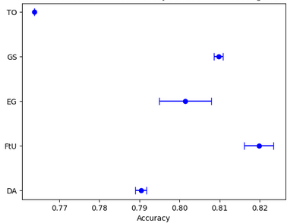
\includegraphics[width=1.0\textwidth, height=1.0\textwidth]{accuracy.png}
    \label{fig:acc_alg}
    \caption{Min-Max accuracy for each fairness algorithm}
\end{figure}

There are some considerations that can be made about the accurencies presented:

\begin{itemize}

    \item The accuracy value for the Threshold Optimizer algorithm is always 0.7673 as showed in the table \cref{fig:results}.

    \item The algorith that leads to the minimum variance in the accuracy results for the two models considered is the Grid Search.

    \item The algorithm that leads to the maximum variance in the accuracy values for the two models considered is the Exponentiated Gradient.

    \item The algorithm that leads to the maximum accuracy interval is, as previously already reported, the Fairness through Unawareness algorithm.

\end{itemize}

\subsubsection{Fairness Values Grouped by Fairness Algorithm}

Similarly, for each fairness algorithm, the minimum and maximum fairness values are presented. This evaluation allows for an understanding of the fairness outcomes associated with different algorithms, providing a comprehensive view of the trade-offs between accuracy and fairness.

\paragraph{Disparate impact for sex protected attribute}

\begin{figure}[H]
    \centering
    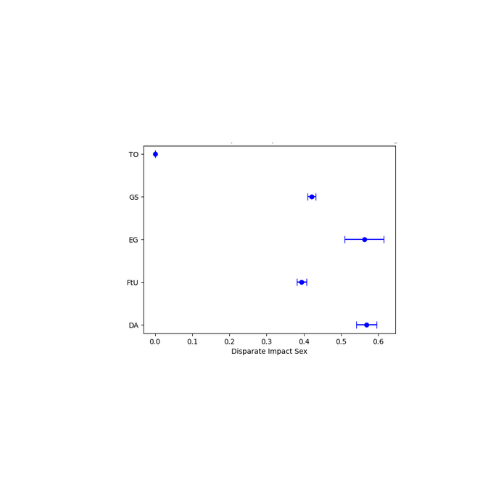
\includegraphics[width=1.0\textwidth, height=1.0\textwidth]{dis.png}
    \label{fig:dis}
    \caption{Min-Max Disparate Impact Metric for Sex protected attributes and for each fairness algorithm}
\end{figure}

\paragraph{Disparate impact for race protected attribute}

\begin{figure}[H]
    \centering
    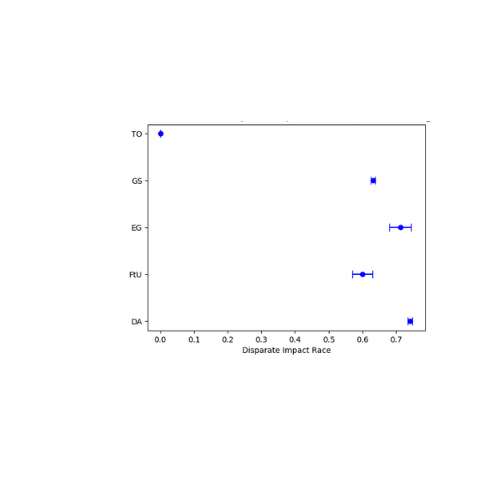
\includegraphics[width=1.0\textwidth, height=1.0\textwidth]{dir.png}
    \label{fig:dir}
    \caption{Min-Max Disparate Impact Metric for Race protected attributes and for each fairness algorithm}
\end{figure}

\paragraph{Demographic parity difference for sex protected attribute}

\begin{figure}[H]
    \centering
    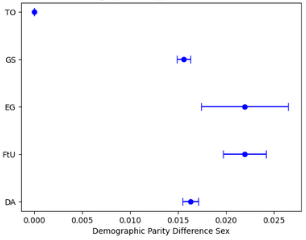
\includegraphics[width=1.0\textwidth, height=1.0\textwidth]{dpds.png}
    \label{fig:dpds}
    \caption{Min-Max Demographic Parity Difference Metric for Sex protected attributes and for each fairness algorithm}
\end{figure}

\paragraph{Demographic parity difference for race protected attribute}

\begin{figure}[H]
    \centering
    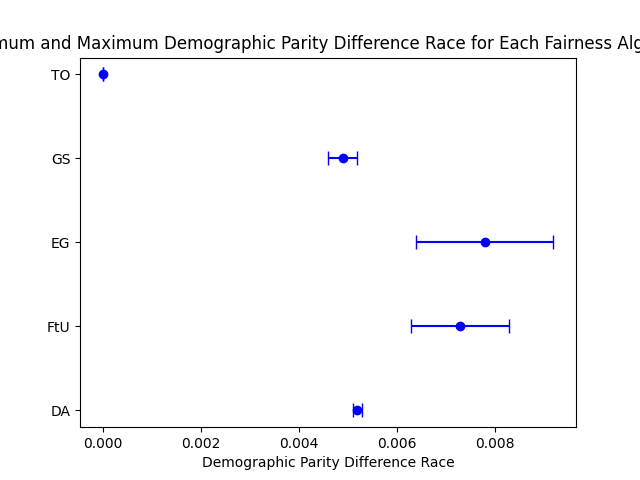
\includegraphics[width=1.0\textwidth, height=1.0\textwidth]{dpdr.png}
    \label{fig:dpdr}
    \caption{Min-Max Demographic Parity Difference for Race protected attributes and for each fairness algorithm}
\end{figure}